\chapter{Visual Navigation Filter}
%\lettrine{I}{n} the present chapter the proposed visual navigation pipeline is presented. 
\vspace{-0.3cm}
\lettrine{I}{n} the present chapter, the visual navigation pipeline proposed in the thesis is presented, utilizing the tools and techniques detailed in Chapter 2 as the foundation for the work.
The algorithm aims at tracking the relative attitude and position (pose) of the target with respect to the chaser using a visible and a thermal monocular camera measurements only. \\
The core of navigation pipeline is an Extended Kalman Filter that provides the pose estimate fusing the information coming from the two sensors. The raw images acquired by the cameras are not fed directly into the filter, but are elaborated in an Image Processing step, which applies pre-processing (if needed) and tracks the relevant point features. The original aspect of the proposed navigation algorithm stays in the filter's innovation computation. The image features and the relative landmark position represent the filter's measurements and pseudo-measurements of the filter. The landmarks position results from the projection of a wireframe model of the target on the image plane according to the available state estimate, thus representing a measure of it. The update step of the filter is then able to correct the pose estimate without reconstructing the pose from the images with algorithms such as the PnP. Additionally, an online estimation of the measurement noise covariance matrix is implemented to avoid modeling errors and adjust for the sensors performance changes due to environmental conditions. \\
A pseudo-code description is presented in \cref{alg:navfilter}, where the implementation of the process is reported. For the sake of clarity a block diagram of the pipeline is also reported in \cref{fig:IPFilter}.

\begin{algorithm}[!h]
\caption{Navigation Filter}\label{alg:navfilter}
\hspace*{\algorithmicindent} \textbf{Input:} Visible and/or thermal image from navigation cameras
\begin{algorithmic}[1]
\State Pre-process the thermal images (histogram equalization)
\State Track the features on the images at $t_k$ given their position in the previous measurements  $t_{k-1}$
\State Propagate the states and the associate covariance from $t_{k-1}$ to $t_k$
\State Project the model landmarks according to the pose provided by the propagated states
\State Compute the filter's innovation: image features position minus landmarks position
\State Compute the Kalman gain and perform the state update (\cref{alg:EKF})
\State Update the estimate of the measurement noise covariance
\end{algorithmic}
\end{algorithm}

Throughout this chapter, the visual navigation filter is presented to provide a detailed insight into the proposed navigation solution. After an introduction on the adopted reference frames, the dynamical model employed by the filter to propagate the states is discussed. The presentation of the measurement model is splitted between the description of the measurement function defined to compute pseudo-measurements and the Image Processing pipeline exploited to detect and track features. Finally, the methods used to estimate the measurement noise covariance matrix and remove outliers are described.

% \lettrine{T}{he} core of the visual navigation pipeline is an Extended Kalman Filter that filters the visual measurements with a simplified relative traslational and rotational dynamic of the system. The measurements fed into the EKF are the output of an Image Processing routine. At each available measurement, the features are tracked given their position in the previous image. At the same time the corresponding features of the available 3D wireframe model of the target are projected onto the image plane. The difference in position between the projected model points and the tracked features on the images represent the measurement innovation, where the model points are the measurements estimated with the filter dynamic, and the tracked features the actual measurements coming from the sensors. An schematic of the architecture is reported in \cref{fig:IPFilter}.\\

\begin{figure}[!h]
    \centering
    \includegraphics[width = \linewidth]{Images/archit.pdf}
    \caption{Visual navigation pipeline architecture}
    \label{fig:IPFilter}
\end{figure}

% The present chapter provides a detailed explanation of the filter. After introducing the reference frames used, the dynamical model inside the filter is presented. Subsequently, the Image Processing workflow, the measurement model and their interface are presented. Finally the noise matrices adaptation method and the outlier rejection algorithm are discussed. 


\section{Reference frames}
\chaptermark{Visual Navigation Filter}
The fundamental reference frames used in the thesis are hereafter presented.\\
The spacecraft absolute position and attitude are expressed in Earth Centered Inertial frame $\mathcal{I}$ (\cref{fig:ECI}). \\
The origin of the Local Vertical Local Horizon ($\mathcal{L}$) frame is the barycenter of the spacecraft, the x axis is directed from the spacecraft radially outward, the z axis is aligned with the normal of the orbit plane and positive along the direction of the angular momentum. The y-axis completes the right-handed triad (\cref{fig:LVLH}).\\
\begin{figure}[!h]
    \begin{subfigure}{0.54\linewidth}
    \includegraphics[width = \linewidth]{Images/ECI.PNG}
    \caption{Earth Centered Inertial reference frame}
    \label{fig:ECI}
    \end{subfigure}\hfill
    \begin{subfigure}{0.43\linewidth}
    \includegraphics[width = \linewidth]{Images/LVLH.PNG}
    \caption{Local Vertical Local Horizon reference frame}
    \label{fig:LVLH}
    \end{subfigure}
    \caption{ECI and LVLH coordinate systems, taken from \cite{alfriend2009spacecraft}}
    \label{fig:orbitrefs}
\end{figure}
The Body frame is instead attached to the spacecraft, having the center in the center of mass of the body. The body frame ($\mathcal{B}$) axes are aligned with the principal axis of inertia of the spacecraft. \\
Finally the sensor coordinate system, the camera frame ($\mathcal{C}$), shall be introduced to describe the position of external elements with respect to the sensor. This coordinate system is described in detail in \cref{sec:cameramodel}.\\
To express in which coordinate system a vector is described, its reference letter is added as subscript. In the case of the LVLH and Body reference frames, as they can be applied both to the chaser and the target, the lowercase letters $c$ and $t$ are added to specify the origin of the system. An example of this notation is reported in \cref{eq:notation}.
\begin{equation}
\label{eq:notation}
    \vect{r}_C = \vect{A}_{C/Bc} \vect{A}_{Bc/I} \vect{r}_I
\end{equation}
The generic vector $\vect{r}$ is mapped from the Earth Centered Inertial to the Camera frame by mean of two consecutive rotations expressed in terms of Direct Cosine Matrices $\vect{A}$. For elements expressing the transformation between the two reference frames, such as rotation matrices or quaternions, the convention used is the one reported in \cref{eq:notation}. $\vect{A}_{Bc/I}$ represents the chaser body frame ($Bc$) expressed in the inertial reference frame ($I$), and $\vect{A}_{C/Bc}$ represents the camera frame expressed in the chaser body reference frame.

\section{Dynamical model}
\chaptermark{Visual Navigation Filter}
As the filter estimates the 6 degrees of freedom pose of the target, the dynamical model includes both the translational and the rotational dynamic of the relative motion. 
%Specifically, the states of the filter are comprised of the position and velocity of the target in the chaser reference frame, a three-element attitude error state and angular velocity of the target body frame expressed in the chaser body frame.
Specifically, the states of the filter are comprised of the position and velocity of the target in the chaser LVLH frame, a three-element attitude error expressed in MRP and the angular velocities of the target body frame expressed in the chaser body frame. 
In the present section the state propagation model is detailed. During the discussion, to express the target position in the chaser's body frame ($\vect{x}_{Lc} = [x_{Lc} \ y_{Lc} \ z_{Lc}]$) and the relative attitude ($q_{Bt/Bc}$), the subscripts indicating the reference frames are avoided for the sake of brevity.
\subsection{Translational dynamic}
The relative motion between two spacecrafts is an intrinsically non-linear problem. An extensive derivation of the differential equation describing the target motion expressed in the chaser LVLH frame is reported in \cite{alfriend2009spacecraft}, resulting in the general nonlinear equations of relative motion:

\begin{equation}
\label{eq:alfr}
\begin{split}
    \Ddot{x}-2\dot{f}_c \dot{y} - \Ddot{f}_c y - \dot{f}_c^2 x &= - \dfrac{\mu (r_c + x)}{[(r_c + x)^2 + y^2 + z^2]^{3/2}} + \dfrac{\mu}{r_c^2} +  d_R\\
    \Ddot{y}+2\dot{f}_c\dot{x}+\Ddot{f}_c x - \dot{f}_c^2 y &= - \dfrac{\mu y}{[(r_c + x)^2 + y^2 + z^2]^{3/2}} + d_T\\
    \Ddot{z}& = - \dfrac{\mu z}{[(r_c + x)^2 + y^2 + z^2]^{3/2}} + d_N\\
    \end{split}
\end{equation}

where $f_c$ and $r_c$ represent the true anomaly and the radius of the chaser respectively, and $[d_R,d_T,d_N]$ the differential perturbing acceleration in the radial, tangential and normal directions. \\
In the context of spacecraft rendezvous, Clohessy and Wiltshire \cite{clohessy1960terminal} proposed a linear form of the equations of relative motion by neglecting all perturbations considering only the first order terms of the Taylor expansion of \cref{eq:alfr} \cite{sullivan2017comprehensive}. This model of motion is here selected for the translational dynamic of the filter. The selection of such a simplified model is justified by the short measurements update intervals  of close proximity operations (in the order of seconds) and by the quasi-circular orbit of space debris in LEO orbits. In case those assumption are not applicable more complex models such as the Yamanaka-Ankersen \cite{yamanaka2002new} are advised. 
The Clohessy-Wiltshire (CW) linearized equations of unperturbed relative motion are reported in \cref{eq:CW}.
\begin{equation}
    \label{eq:CW}
    \begin{split}
        \Ddot{x}-2n\dot{y}-3n^2x & = 0\\
        \Ddot{y}+2n\dot{x} & = 0\\
        \Ddot{z}+n^2z& = 0
    \end{split}
\end{equation}
where $n$ indicates the mean motion of the chaser. 
% These equations can be rewritten in state-space form as:
% \begingroup
% \renewcommand{\arraystretch}{1}
% \begin{equation}
%     \begin{bmatrix}
%         \dot{x} \\ \dot{y} \\ \dot{z} \\ \Ddot{x} \\ \Ddot{y} \\ \Ddot{z} 
%     \end{bmatrix}= \begin{bmatrix}
%         0 & 0 & 0 & 1 & 0 & 0\\
%         0 & 0 & 0 & 0 & 1 & 0 \\
%         0 & 0 & 0 & 0 & 0 & 1 \\
%         3n^2 & 0 & 0 & 0 & 2n & 0 \\
%         0 & 0 & 0 & -2n & 0 & 0 \\
%         0 & 0 & -n^2 & 0& 0 & 0\\
%     \end{bmatrix}\begin{bmatrix}
%        x \\ y \\ z \\ \dot{x} \\ \dot{y} \\ \dot{z} 
%     \end{bmatrix}
% \end{equation}
% \endgroup
The state transition matrix of the CW equations can be computed analitically and is reported in \cref{eq:CWSTM}, where $c_{nt}$ and $s_{nt}$ indicates $cos(nt)$ and $sin(nt)$ respectively \cite{alfriend2009spacecraft}.
\begingroup

\begin{equation}
\label{eq:CWSTM}
%\renewcommand*{\arraystretch}{1.2}
\Phi_{CW} = \begin{bmatrix}
4-3c_{nt} & 0 & 0 &\dfrac{s_{nt}}{n} & \dfrac{2}{n}-\dfrac{2c_{nt}}{n} & 0\\[0.5em]
-6nt+6s_{nt} & 1 & 0 & -\dfrac{2}{n}+\dfrac{2c_{nt}}{n} & \dfrac{4s_{nt}}{n}-3t & 0\\[0.5em]
0 & 0 & c_{nt} & 0& 0& \dfrac{s_{nt}}{n}\\[0.5em]
3ns_{nt} & 0 & 0 & c_{nt} & 2s_{nt} & 0 \\[0.5em]
-6n+6nc_{nt} & 0 & 0 & -2s_{nt} & -3+4c_{nt} & 0 \\[0.5em]
0 & 0 & -ns_{nt} & 0 & 0 & c_{nt}
\end{bmatrix}
\end{equation}
\endgroup
\subsection{Rotational dynamic}
The target absolute angular accelerations cannot be determined in an uncooperative scenario; the model here used for attitude dynamics assumes constant small relative angular velocities, as proposed in \cite{sharma2017reduced, geyer2021relative}. A quaternion parametrization is adopted, formalized in \cref{eq:dyn1,eq:dyn1_1}.

\begingroup
\renewcommand{\arraystretch}{0.8}
%\begin{equation}
    
    \begin{align}
    \label{eq:dyn1}
        \dot{\vect{q}} &=\frac{1}{2}\Omega(\boldsymbol{\omega}) \vect{q} = \begin{bmatrix}
            \omega \\ 0
        \end{bmatrix} \otimes \vect{q}\\\label{eq:dyn1_1}
        \dot{\boldsymbol{\omega}}&= \vect{0}
    \end{align}
%\end{equation}
\endgroup

where $\vect{q} = [q_1\ q_2\ q_3\ q_4]^T$, with $q_4$ as scalar part, is the target body frame expressed in the chaser body frame, and $\boldsymbol{\omega}$ the relative angular velocities vector. $\Omega(\boldsymbol{\omega})$ is a 3$\times$4 matrix defined as:

\begin{equation}
    \label{eq:dyn2}
    \Omega(\boldsymbol{\omega}) = \begin{bmatrix}
        -[\boldsymbol{\omega}\times] & \boldsymbol{\omega}\\
        -\boldsymbol{\omega}^T & 0
    \end{bmatrix}
\end{equation}

where $[\boldsymbol{\ \cdot \ }\times]$ indicates the skew-symmetric matrix. As the filter exploits the multiplicative representation of the quaternion error (\cref{sec:MEKF}), it is necessary to derive the attitude dynamical model as function of the three-element error vector $\vect{a}_p$ expressed in MRP. 
This can be obtained by substituting  \cref{eq:dyn1} in the time derivative of \cref{eq:q2mrp}:
\begin{equation}
    \label{eq:apder}
    \begin{split}
        \dot{\vect{a}}_p & = \dfrac{4}{1+q_4}\dot{\bar{\vect{q}}} - \dfrac{4}{(1+q_4)^2}\dot{q_4}\bar{\vect{q}}\\
        & = \Big(-\dfrac{1}{2}[\boldsymbol{\omega}\times] + \dfrac{1}{8}\boldsymbol{\omega}\cdot\vect{a}_p\Big)\vect{a}_p+\Big(1-\dfrac{1}{16}\vect{a}_p^T\vect{a}_p\Big)\boldsymbol{\omega}\\
        & = -\dfrac{1}{2}[\boldsymbol{\omega}\times]\vect{a}_p+\boldsymbol{\omega}\\
    \end{split}
\end{equation}
\cref{eq:apder,eq:dyn1_1} represent the differential equations of the attitude dynamical model. 
% Those can be rewritten in state space form as:
% \begingroup
% \renewcommand{\arraystretch}{1}
% \begin{equation}
%     \begin{bmatrix}
%         \dot{\vect{a}}_p \\ \dot{\boldsymbol{\omega}}
%     \end{bmatrix}= \begin{bmatrix}
%         -\dfrac{1}{2}[\boldsymbol{\omega}\times] & \vect{I} \\
%         \vect{0} & \vect{0} 
%     \end{bmatrix}\begin{bmatrix}
%         \vect{a}_p \\ \boldsymbol{\omega}
%     \end{bmatrix}
% \end{equation}
% \endgroup
In this case, the State Transition Matrix $\Phi_{att}$ cannot be computed analytically but requires numerical computation. The approach suggested in \cite{tweddle2015relative} is to use the exponential matrix, and, as no difference in terms of accuracy was found comparing this method with the variational approach, it is used for the computation of the STM. \\

The complete rotational-translationa propagation model can be expressd in compact form as:
\begin{equation} 
    \begin{pmatrix}
    \dot{\vect{x}} \\  \ddot{\vect{x}} \\  \dot{\vect{a}}_p \\ \dot{\boldsymbol{\omega}}\end{pmatrix} = \begin{bmatrix}
        \Phi_{CW} & \vect{0} \\ \vect{0} & \Phi_{att}
    \end{bmatrix}\begin{pmatrix}
    \vect{x}\\  \dot{\vect{x}} \\  \vect{a}_p \\ \boldsymbol{\omega}\end{pmatrix}
\end{equation}


\section{Measurement model}
\label{sec:mesmodel}
\chaptermark{Visual Navigation Filter}
The measurement model is a function that transforms the filter states to the estimates of the measurements coming from the sensors. In the here treated context, this implies mapping the landmarks of the target known 3D model, expressed in the target body frame, to their estimated position on the image plane.
The measurement function building can be conceptually divided in three steps, namely the transformation of the features position from the target body frame to the camera frame ($h_1$), a second step of projection of the points on the image plane ($h_2$), and  finally the conversion from homogeneous to Cartesian coordinates ($h_3$). \\
The first step is formalised in \cref{eq:meas1}.
\begin{equation}
\label{eq:meas1}
    \vect{f}_C = h_1(\vect{x}_{Lc},\vect{a}_p) =\vect{A}_{C/Bc}(\vect{A}(\vect{q}(\vect{a}_p)\otimes\vect{q}_{Bt/Bc})^T\vect{f}_{Bt} + \vect{A}_{Bc/I}\vect{A}_{I/Lc}\vect{x}_{Lc}) - \vect{A}_{C/Bc}\vect{t}_{Bc}
\end{equation}
where $\vect{f}_C$ is a generic landmark position in the camera reference frame, $\vect{f}_{Bt}$ its position in the target body frame and $\vect{t}_{Bc}$ the position of the camera in the chaser body frame. The transformation matrices $\vect{A}_{Bc/I}$ and $\vect{A}_{I/Lc}$ can be determined because the position and attitude of the chaser in the inertial frame are assumed to be known. In real applications, the DCM $\vect{A}_{C/Bc}$ and the translation vector $\vect{t}_{Bc}$ have different values for different cameras, as they are necessarily placed in different positions onboard the chaser. However, within the current application both the thermal and the visible cameras are assumed to lie in the center of the chaser mounted with the same attitude. This assumption is not realistic but does not entail any difference to the navigation pipeline. \\
The MRP attitude error $\vect{a}_p$, used to retrieve the estimated attitude of the chaser in the attitude reference frame, and the target position in the chaser LVLH frame $\vect{x}_{Lc}$ are the states dependent on the measurements. As expected, the velocity and angular rate do not appear, as they do not provide any information on the features position at a given time. 
The second step corresponds to the projection of the points to the image plane according to the pinhole camera model described in \cref{sec:cameramodel}:
\begin{equation}
    \label{eq:h2}
    \vect{f}^h = h_2(\vect{f}_C) = \vect{K}\vect{f}_C
\end{equation}
where $\vect{f}^h = [f_x^h \ f_y^h \ f_z^h]^T$ indicates the feature position on the image plane expressed in homogeneous coordinates. As the visible and thermal cameras are assumed to be coincident, the intrinsic camera matrix is the only factor that distinguishes the two sensors within the context of the measurement function.\\
%As in this equation appears the intrinsic camera matrix, this step is the only step characterising the sensor used for the measurement, changing the parameters of the intrinsic matrix according to the physical proprieties of the visible and thermal cameras.\\
The final step consists in the non-linear transform between the homogeneous and Cartesian coordinates:
\begin{equation}
    \label{eq:h3}
    \vect{f} = h_3(\vect{f}^h) = \left\{ \begin{array}{c}
         \dfrac{f_x^h}{f_z^h}  \\[10pt]
         \dfrac{f_y^h}{f_z^h}  
    \end{array}\right.
\end{equation}
Combining the defined equations according the definition of \cref{eq:EKF2}, and defining the output pseudo-measurements $\vect{y}$ as the landmark position $\vect{f}$, the full measurement function can be defined as:
\begin{equation}
    \vect{y} = h_3(h_2(h_1(\vect{x}_{Lc},\vect{a}_p)))
\end{equation}
The resulting measurement function is non-linear, therefore the Jacobian of the function has been computed with respect to all the filter states to be compatible with the EKF formulation. Since it is not function of the velocity or the angular rates, the columns of the Jacobian associated to those states will be zeros. 

\section{Image Processing pipeline}
\chaptermark{Visual Navigation Filter}
\label{sec:IP}
The scope of the image processing pipeline is to provide the image features location and their relation to the wireframe model points. A flow diagrams of the IP pipeline is reported in \cref{fig:IP}. \\
The features position on the image acquired at time $t_k$ are the output of the Lucas Kanade tracker, using the results obtained at time $t_{k-1}$ as initial condition. 
%As the features are tracked along different images, their association with the respective model landmark is known. 
As the features are tracked along different images, the information about their correlation with the model landmarks is maintained, avoiding the need of a matching process at each filter step.  
To remove either spurious associations or errors collected during the tracking step, a RANSAC routine is added to remove possible outliers. If the number of features after the outlier rejection is over a defined threshold $k$, then the IP step can be considered satisfactory and the information acquired is used in the filter to refine the estimated pose. \\
\begin{figure}[!h]
    \centering
    \includegraphics[width = \linewidth]{Images/IPstep.pdf}
    \caption{Image processing pipeline architecture}
    \label{fig:IP}
\end{figure}

However, as explained in \cref{sec:features}, the number of features strictly decreases over time, requiring a re-initialization step. \\
In the re-initialization the problem of redefining the correlations between image features and model landmarks arises. A possible solution is to perform a brute-force RANSAC association by randomly sampling the entire set of image features and model points until the correct correspondences are extracted and the associations are computed.  Given the large number of features, the number of iterations required to ensure a good probability of success would make the algorithm prohibitive for real-time applications. \\
The solution here proposed exploits the information about the image-to-map correlation available before the re-initialization process to limit the brute-force RANSAC search region.  The steps of the implemented solution are described in pseudocode in \cref{alg:IP}. \\ 
Given the output of the RANSAC outlier rejection routine, the homography matrix mapping the model landmarks to the respective image features is computed. To combine those two steps is equivalent to applying the Golden Standard algorithm (\cref{sec:RANSAC}), thus providing the best estimate of the projection of the landmarks onto image features. At this point, it is possible to use the retrieved projective transformation matrix to map all model landmarks to where their corresponding image feature is expected to be located. Once detected the new features from the image, it is reasonable to assume that the associated landmarks are  restricted to a limited region about their location. When performing the RANSAC polling, only the landmarks within a certain distance $d_{max}$ from the respective extracted feature are considered. The more the search region dimension is extended, the more the method is robust to estimation errors, although increasing the computational burden. The search region is therefore to be tuned to reach the desired trade-off between robustness and computational time. 

\begin{algorithm}
\caption{IP re-initialization algorithm}\label{alg:IP}
\begin{algorithmic}[1]
\State Given: a vector of image features locations $\vect{f}_a^i$ and the associated projected model points locations $\vect{f}_a^m$, subset of all model landmarks on the image plane $\vect{F}_a^m$
\State With DLT, compute the homography s.t. $\vect{f}_a^i \simeq \vect{H}\vect{f}_a^m$
\State Trasform all the model points s.t. $\vect{F}_b^m = \vect{H}\vect{F}_a^m$ 
\State Detect a new set of features $\vect{f}_b^i$ from the image 

\While{$n_{iter}<n_{max}$}
    \State Randomly select 4 elements from $\vect{f}_b^i$
    \State Randomly select 4 elements from the subset of  $\vect{F}_b^m$ s.t. $\parallel \vect{F}_b^m - \vect{f}_b^i \parallel \leq d_{max}$
    \State Compute the homography matrix between the selected points and select the inliers \quad $\vect{f}_b^m$ of the model 
    \State Count the number inliers $\varepsilon$ of the fitted model 
    \If{$\varepsilon > \varepsilon_{max}$}
    \State Update $\varepsilon_{max}$ and save $\vect{f}_b^i$ and $\vect{f}_b^m$ as the re-intialized features
    \EndIf
\EndWhile
\end{algorithmic}
\end{algorithm}

The IP pipeline is almost identical for the visible and thermal spectra. The only difference is the application of the CLAHE contrast equalization to the thermal image. Because of the overall lack of contrast of thermal images, its enhancement is beneficial for the features identification process \cite{rondao2020benchmarking}. 

%\mycomm{create figure with points to make better understand the steps}

\subsection{Feature detector trade-off}
The selection of the feature detector is based on a trade-off performed between different methods. The methods investigated include both blob detectors (SIFT, SURF) and corner detectors (BRISK, FAST, ORB). For all those methods, the formulatio implemented in the Computer Vision toolbox of MATLAB is here adopted.\\
The trade-off is performed against merit-criteria tailored for the thesis applications. As all methods can detect a satisfactory amount of features, given the suitable tailoring of their parameters, they are evaluated on the quality of the features detected in terms of tracking: the more a method can detect features that are reliably tracked along different frames (moving coherently with the associated point on the rigid body) the less re-initialization steps are required, thus providing a positive contribution to the navigation pipeline timeliness.  To achieve this evaluation, the extracted features are tracked along 60 consecutive frames, eliminating outliers at each step. This procedure is executed 100 times on a database of 400 images, starting each run with a different initial frame to avoid test the methods on different point of views of the target. \\
The averaged results obtained over 100 runs are reported for the different methods in \cref{fig:ntracking}.

\begin{figure}[!h]
     \centering
     \begin{subfigure}[b]{0.46\textwidth}
         \centering
         \includegraphics[width=\textwidth]{Images/VISTracking.eps}
         \caption{Visible images}
         \label{fig:trackingvis}
     \end{subfigure}
     \hfill
     \begin{subfigure}[b]{0.46\textwidth}
         \centering
         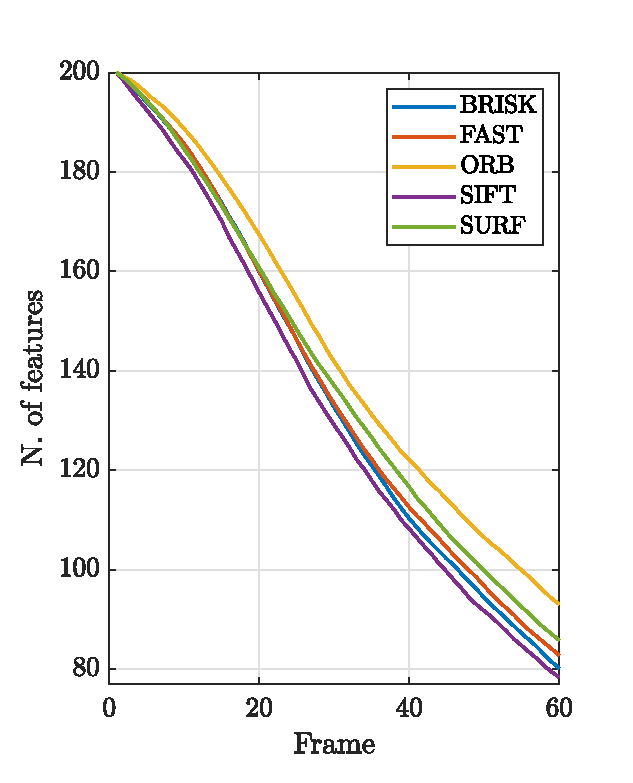
\includegraphics[width=\textwidth]{Images/TIRTracking.eps}
         \caption{Thermal images}
         \label{fig:trackingtir}
     \end{subfigure}
        \caption{Number of features tracked along different frames for visible and thermal images}
        \label{fig:ntracking}
\end{figure}


For both visible and thermal images the best method results to be ORB, as it identifies more reliable features traceable for longer times. It can also be observed an overall difference in performances between the visible and thermal case, as TIR images present a faster feature drop rate. At a first analysis this results seemed counter-intuitive as in the thermal images the shadowing problem does not arise, thus it is expected to maintain a higher number of features over time with respect the VIS images, which are affected by that problem. The reason behind the TIR spectrum lower performances of the TIR spectrum is the spurious association of the features to the model points after the detection, given by the higher noise level in the image and the adopted simplified thermal model. Along the tracking process this outliers are then rejected, justifying the results obtained in \cref{fig:trackingtir}.\\
The computation time required for the feature detection process is a second merit-criterion considered because a lightweight method would ease future onboard testing of the algorithm. \cref{fig:ndetect} shows results for both the visible and thermal case. In both spectra the FAST and ORB methods outperform the others, making the ORB detection the overall best solution for this work application.\\
It should be noted that the trade-off performed is specific to the application and does not generally apply as a benchmark for feature detector methods.

\begin{figure}[!h]
     \centering
     \begin{subfigure}[b]{0.46\textwidth}
         \centering
         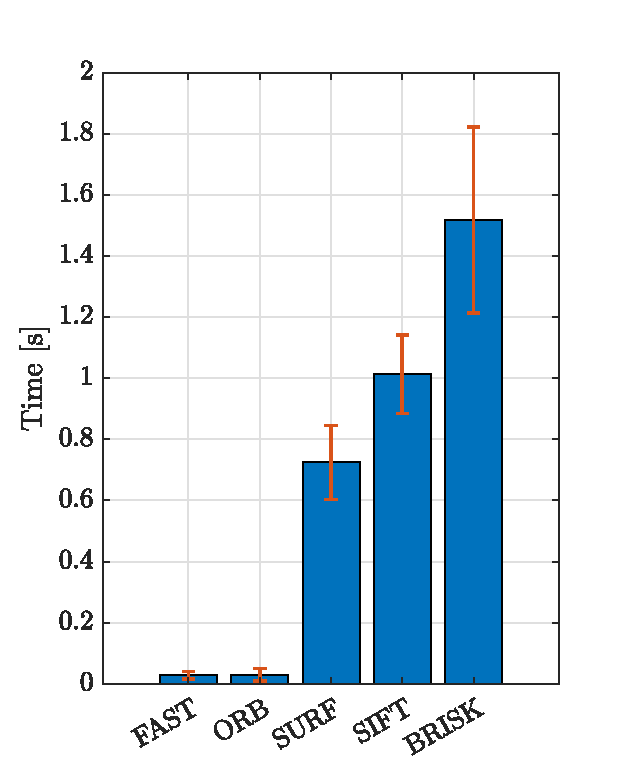
\includegraphics[width=\textwidth]{Images/VISTimesDetect.eps}
         \caption{Visible images}
         \label{fig:detectvis}
     \end{subfigure}
     \hfill
     \begin{subfigure}[b]{0.46\textwidth}
         \centering
         \includegraphics[width=\textwidth]{Images/TIRDetectTime.eps}
         \caption{Thermal images}
         \label{fig:detecttir}
     \end{subfigure}
        \caption[Time required for the feature detection process]{Average time required on the feature detection process for the visible and thermal images over 100 images}
        \label{fig:ndetect}
\end{figure}


\section{Measurement noise matrix adaptation}
\chaptermark{Visual Navigation Filter}
As described in \cref{sec:mesmodel} the features' position on both the visible and thermal images are the measures of the filter. In the framework of the Kalman filter it is necessary to accurately model the measurement noise to avoid degradation of the filter performances or divergence from the ground truth. For navigation cameras this can result in a challenging task, as the noise associated to the detected features is influenced both by the quality of the sensor and by the external environmental conditions; aspects such as either the illumination condition or the chaser-target distance could in fact vary the noise associated to the image features.\\
To tackle this issue the residual-based adaptive estimation of the measurement noise covariance matrix $\vect{R}$ proposed in \cite{akhlaghi2017adaptive} is implemented.\\
The filter residual is defined as the difference between the measurements and the pseudo-measurements of the updated state:
\begin{equation}
    \boldsymbol{\varepsilon}_k = \vect{y}_k - \vect{H}_k \vect{x}_k^+
\end{equation}
As demonstrated in \cite{akhlaghi2017adaptive} the estimate of the residual covariance can be expressed as:
\begin{equation}
    \hat{\boldsymbol{C}}_k = E(\boldsymbol{\varepsilon}_k \boldsymbol{\varepsilon}_k^T) = \hat{\vect{R}}_k - \vect{H}_k \vect{P}_k^- \vect{H}_k^T
\end{equation}
Indicating with $\ \hat{\cdot} \ $ the estimated values. The definition for the estimate of $\vect{R}$ at each step becomes:
\begin{equation}
\label{eq:R_est}
    \hat{\vect{R}}_k = E(\boldsymbol{\varepsilon}_k \boldsymbol{\varepsilon}_k^T) + \vect{H}_k \vect{P}_k^- \vect{H}_k^T
\end{equation}
The expected value of the residual covariance $E(\boldsymbol{\varepsilon}_k \boldsymbol{\varepsilon}_k^T)$ can be approximated by averaging $\boldsymbol{\varepsilon}_k \boldsymbol{\varepsilon}_k^T$ over a sliding window of dimension $N$ as:
\begin{equation}
    E(\boldsymbol{\varepsilon}_k \boldsymbol{\varepsilon}_k^T) = \dfrac{1}{N} \sum_{k=1}^N \boldsymbol{\varepsilon}_k \boldsymbol{\varepsilon}_k^T
\end{equation}
To avoid saving all residuals over the sliding window, a forgetting factor $\alpha$ is introduced to adaptively estimate the measurement noise covariance matrix, rewriting \cref{eq:R_est} as:
\begin{equation}
\label{eq:R_est1}
    \hat{\vect{R}}_k = \alpha\vect{R}_{k-1}  + (1-\alpha)(\boldsymbol{\varepsilon}_k \boldsymbol{\varepsilon}_k^T + \vect{H}_k \vect{P}_k^- \vect{H}_k^T)
\end{equation}
The lower the value of $\alpha$, the more the estimation of $\vect{R}$ depends on the current residual, although the estimate would be subject to fluctuations due to noise within the residuals. The forgetting factor should then be tuned to obtain the desired results from the adaptation.

\section{Outliers rejection}
\chaptermark{Visual Navigation Filter}
Although an outlier rejection method is already introduced in the Image Processing pipeline, it is convenient to discard the noisiest measurements to enhance the performances and the stability \cite{civardi2021small}.\\
As it is assumed that the measurements are affected by known Gaussian noise, a null-hypothesis test is performed to check whether the measurements are in accordance with the assumed model.  As highlighted in \cite{tweddle2015relative}, the square of the Mahalanobis distance ($\gamma_k$) of the innovation can be exploited as performance metric for the null-hypothesis:

\begin{equation}
    \gamma_k = M^2_k = \vect{d}_k^T \vect{S}_k^{-1} \vect{d}_k
\end{equation}

%where the innovation $\vect{d}_k$ is defined as:
where $\vect{d}_k$ is the innovation, $\vect{S}_k$ its covariance matrix and $M_k$ the Mahalanobis distance. The innovation is defined as: 
\begin{equation}
    \vect{d}_k = \vect{y}_k - \vect{H}_k \vect{x}_k^-
\end{equation}
And the associated covariance $\vect{S}_k$ as:
\begin{equation}
    \vect{S}_k = \vect{H}_k \vect{P}_k^- \vect{H}_k^T + \vect{R}
\end{equation}

Under the assumption that the null-hypothesis is true, i.e.the error is Gaussian distributed, $\gamma_k$ should be Chi-square distributed with degrees of freedom equal to the dimensionality of the innovation vector. 
To remove possible outliers a gating method is applied, excluding all measurements which are bigger than a threshold $\chi_\alpha$ defined so that \cref{eq:chisq} is true.
\begin{equation}
    \label{eq:chisq}
    P(\gamma_k>\chi_\alpha) = \alpha
\end{equation}

\cref{eq:chisq} expresses that the probability of a randomly selected $\gamma_k$ to be higher than $\chi_\alpha$ is equal to $\alpha$. The value of $\alpha$ is selected to be 0.05. Such value ensures that the noisiest measurements are removed without excluding inliers.\\
That approach for outliers rejection enables both to remove possible outliers and to remove from the measurement vector the most noisy values, thus enhancing the filter's performances.